% Taylor & Francis LaTeX template for authors (Interact layout + APA reference style)
% source: https://www.overleaf.com/latex/templates/taylor-and-francis-latex-template-for-authors-interact-layout-plus-apa-reference-style/jqhskrsqqzfz

\documentclass[]{./cls/interact}

% Template Preamble

\usepackage{epstopdf}				% To incorporate .eps illustrations using PDFLaTeX, etc.
\usepackage[caption=false]{subfig}		% Support for small, `sub' figures and tables
%\usepackage[nolists,tablesfirst]{endfloat}	% To `separate' figures and tables from text if required
%\usepackage[doublespacing]{setspace}		% To produce a `double spaced' document if required
%	\setlength\parindent{24pt}		% To increase paragraph indentation when line spacing is doubled

% Citation support using apacite.sty. 
\usepackage[natbibapa,nodoi]{apacite}					% Citation support using apacite.sty. 
\setlength\bibhang{12pt}						% To set the indentation in the list of references using apacite.sty. 
\renewcommand\bibliographytypesize{\fontsize{10}{12}\selectfont}	% To set the list of references in 10 point font using apacite.sty. 

% Theorem-like structures provided by amsthm.sty
\theoremstyle{plain}				
\newtheorem{theorem}{Theorem}[section]
\newtheorem{lemma}[theorem]{Lemma}
\newtheorem{corollary}[theorem]{Corollary}
\newtheorem{proposition}[theorem]{Proposition}

\theoremstyle{definition}
\newtheorem{definition}[theorem]{Definition}
\newtheorem{example}[theorem]{Example}

\theoremstyle{remark}
\newtheorem{remark}{Remark}
\newtheorem{notation}{Notation}

% Custom Preamble

% Important packages
\usepackage{hyperref}	% automatic pdf outline and citations hyperlinks
\usepackage{placeins} 	% for FloatBarrier

% Paths
\newcommand{\pathBIB}{./bib}
\newcommand{\pathFIG}{./figures}
% Paths for work in progress versions
%\newcommand{\pathFIG}{../output/graphs} 	% pools from my R output folder
%\newcommand{\pathBIB}{../../statsLib}		% pools from my bibliography

% Macros
\newcommand{\norm}[1]{\left\lVert#1\right\rVert} % for l2 norm in equations

% Begin Manuscript
\begin{document}

\articletype{SUPPLEMENTARY MATERIAL}	% Specify the article type or omit as appropriate

% Manuscript details
\title{High Dimensional Imputation for the Social Sciences: A Comparison of State-of-the-Art Methods}

\author{
\name{
	Edoardo Costantini\textsuperscript{a} \thanks{CONTACT Edoardo Costantini. Email: e.costantini@tilburguniversity.edu},
	Kyle M. Lang\textsuperscript{a},
	Tim Reeskens\textsuperscript{b}, and
	Klaas Sijtsma\textsuperscript{a}
	}
\affil{
	\textsuperscript{a}Tilburg University, Department of Methodology and Statistics;
	\textsuperscript{b}Tilburg University, Department of Sociology
	}
}

\maketitle

% Body
\section{Software and other computational details}

The code to run the simulation was written in the R statistical programming language (version 4.0.3). 
All experiments were run using a 2.6 GHz Intel Xeon(R) Gold 6126 processor, 523.78 GB of Memory. The
operating system was Windows Server 2012 R2.
Computations were run in parallel across 30 cores. 
Parallel computing was implemented using the R package \emph{parallel} and to ensure replicability 
of the findings seeds were set using the method by \cite{lecuyer:2002} implemented in the R package 
\emph{rlecuyer}.
Code to run the studies can be found at \url{https://github.com/EdoardoCostantini/imputeHD-comp}.
In the following, each step of the simulation procedure is described in details for both experiments.

\section{Convergence check details}

	Convergence of the imputation models was assessed in a preprocessing step.
	Before running the actual simulation studies, 10 datasets were generated according to each experimental set up.
	Missing values in each dataset were imputed by running 5 parallel imputation chains for each Multiple Imputation 
	method.
	Convergence was checked by plotting the mean of the imputed values for each variable in each stream, against the 
	iteration number.
	In each parallel run, all the MI algorithms run for 250 iterations.
	The imputation algorithms were considered to have converged after 50 iterations, after which 10 imputed data 
	sets were store and used for the subsequent standard complete-data analysis and pooling.
	The only exception was blasso, which required approximately 2000 iterations for convergence.

\section{Ridge penalty cross-validation details}
	The ridge penalty used in the bridge algorithm was fixed across iterations .
	The value used in the simulation was determined by means of cross-validation in a pre-processing phase.
	The grid of possible values for the ridge penalty was $10^{-1}, 10^{-2}, ..., 10^{-8}$.
	For each of 100 data repetitions, bridge imputation was performed with each of the different penalty parameters
	and used to obtain 10 differently imputed datasets.
	For each data replication, the Fraction of Missing Information (FMI) \citep{savaleiRhemtulla:2012} associated with 
	each parameter in the analysis models of interest (see next section for details) was computed and then averaged across 
	repetitions.
	The mean of these average parameter FMIs was used as a composite measure of FMI associated with each ridge penalty
	value.
	Finally, the penalty value with the smallest composite FMI was selected.

\section{Additional Figures}

\subsubsection{Experiment 1: Simulated Data from Multivariate Normal Distribution}

	Figures \ref{fig:exp1bias} and \ref{fig:exp1cir} report the Percentage Relative Bias and Confidence Interval 
	Coverage, respectively, for each parameter estimate in the saturated model described above. 
	In the figures, single horizontal lines, representing the PRB (or CIC) of a parameter estimate for a single 
	variable, combine to form larger horizontal bars giving an aggregate account of how each method performed 
	across multiple variables with missing values.

\begin{figure}
\centering
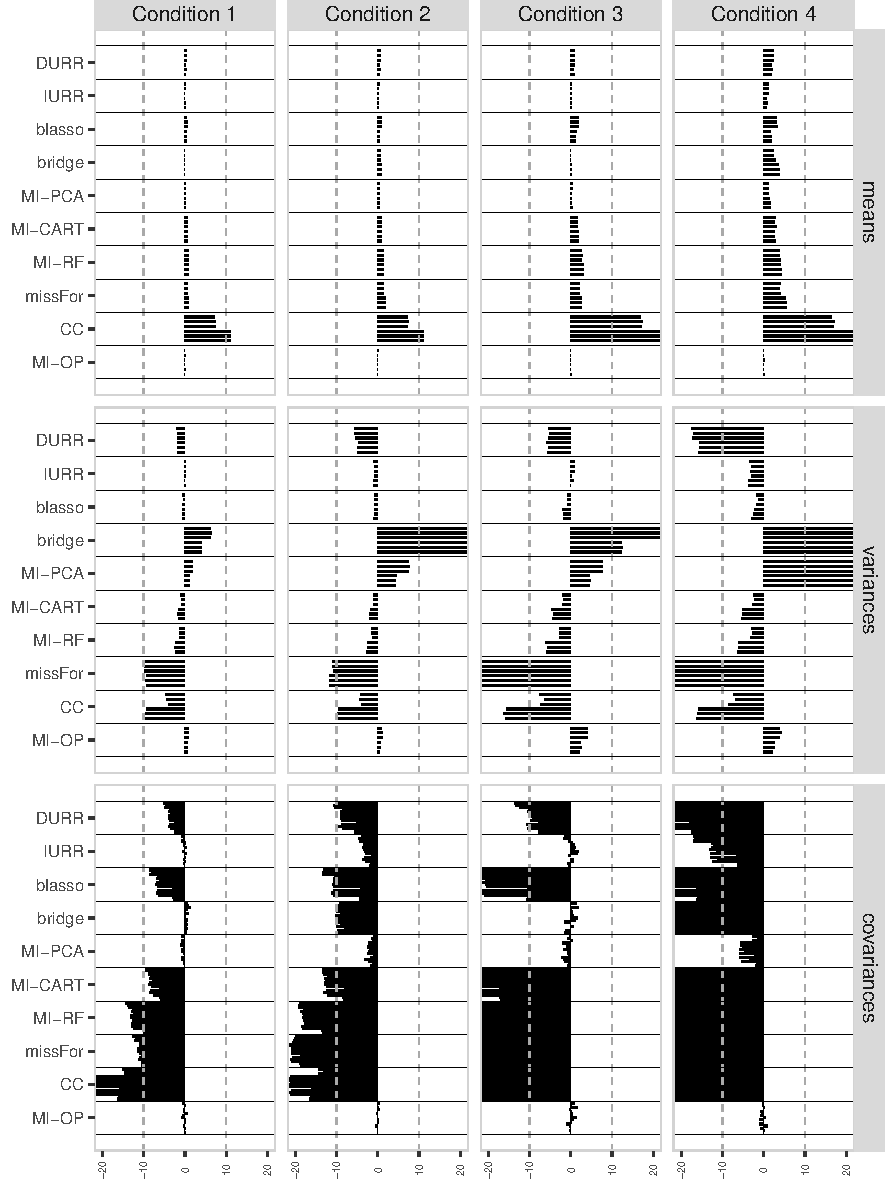
\includegraphics{\pathFIG/exp1_bias.pdf}
\caption{\label{fig:exp1bias}
	Percent Relative Bias (PRB) for item means, variances, and covariances.
	For every method, single horizontal lines, representing the PRB of a parameter estimate on 
	a single variable (or pair of variables), combine to form larger horizontal bars giving an 
	aggregate account of how each method performed across multiple variables with missing values.
	}
\end{figure}

\begin{figure}
\centering
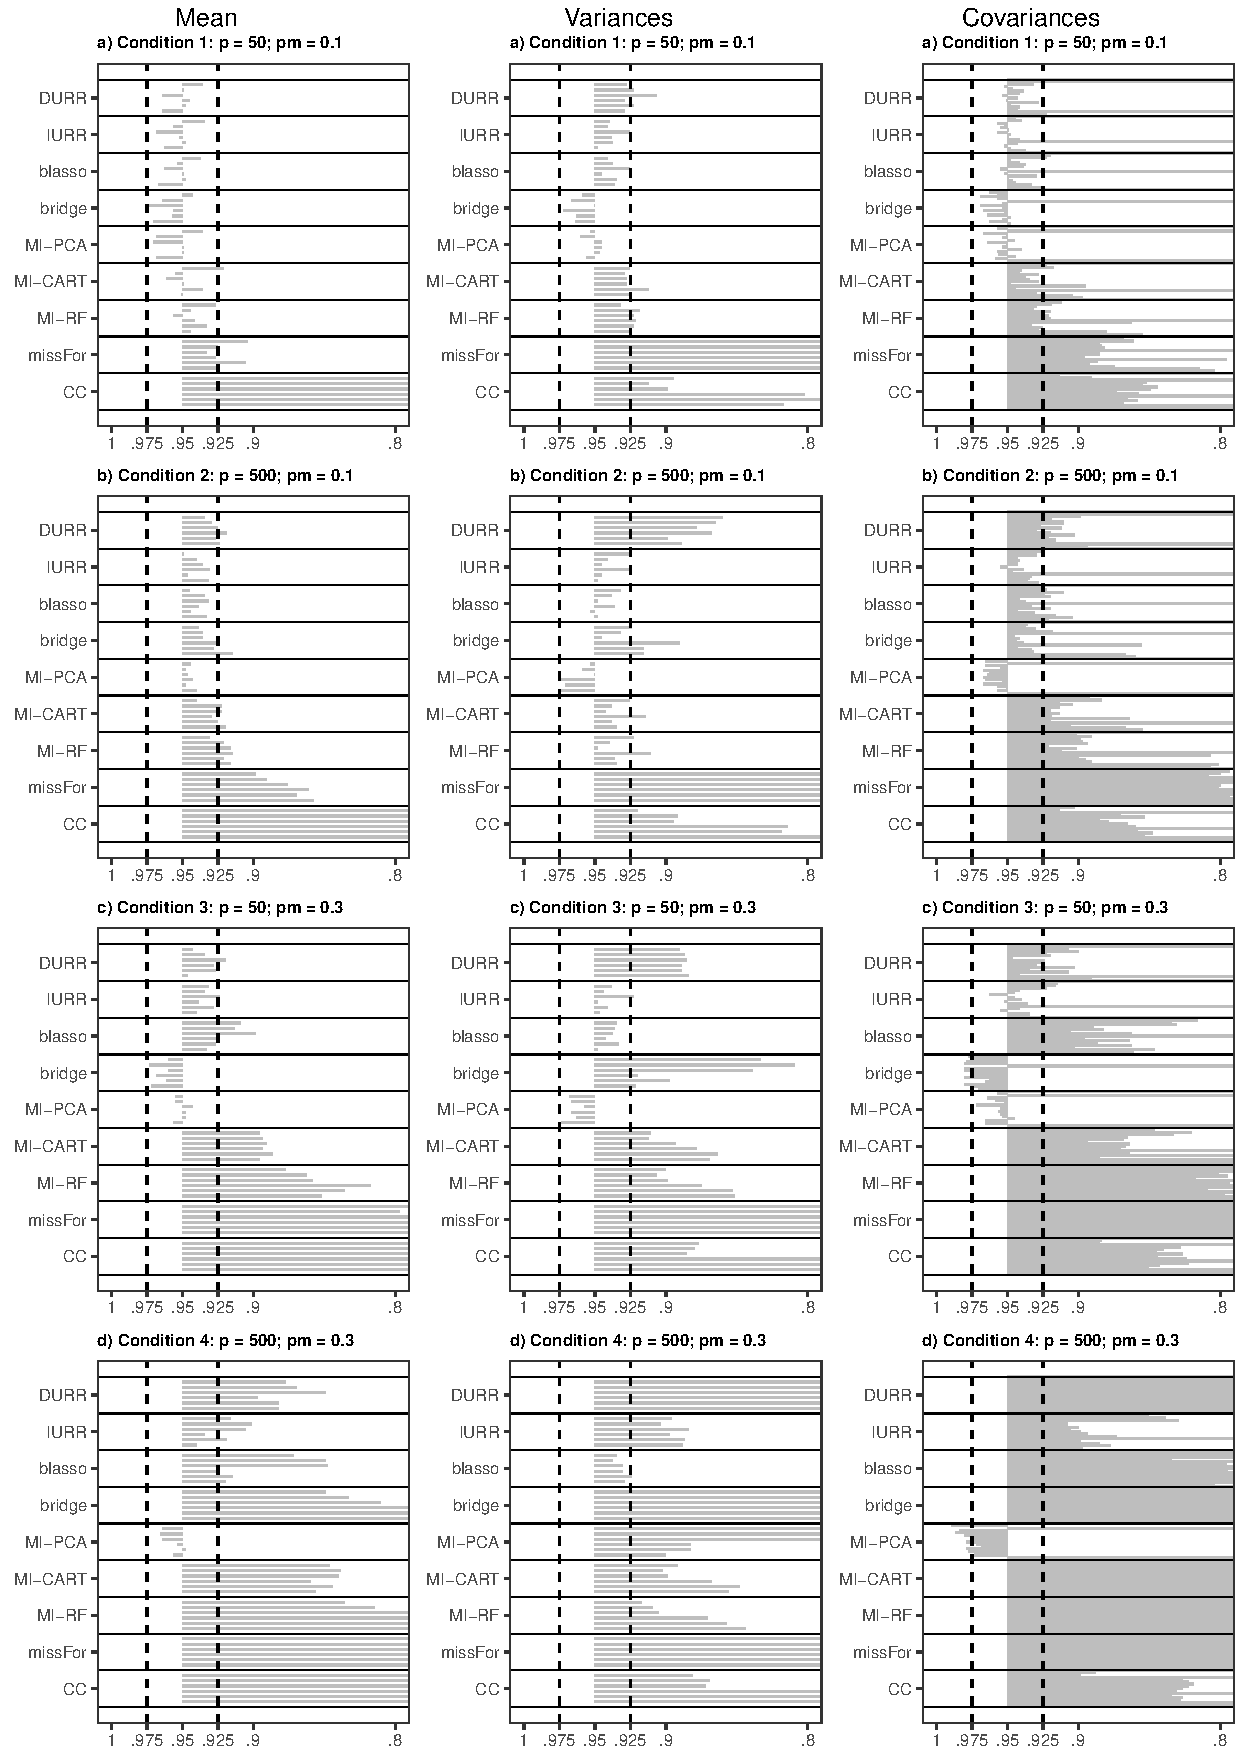
\includegraphics{\pathFIG/exp1_CI.pdf}
\caption{\label{fig:exp1cir}
	Confidence Interval Coverage (CIC) for item means, variances, and covariances. 
	For every method, single horizontal lines, representing the CIC of a parameter estimate on 
	a single variable (or pair of variables), combine to form larger horizontal bars giving an 
	aggregate account of how each method performed across multiple variables with missing values.
	}
\end{figure}

\FloatBarrier

%% EXP 2

\subsection{Experiment 2: Simulated Data with Latent Structure}

	Figures \ref{fig:exp2bias14} and \ref{fig:exp2cir14} report the PRB and CIC of the estimated means, variances, 
	and covariances of the 10 items with missing values in the first four conditions of Experiment 2, 
	the ones characterized by high factor loadings (strong latent structure).
	Figures \ref{fig:exp2bias58} and \ref{fig:exp2cir58} report the same results for the conditions with low
	factor loadings.
	Figure \ref{fig:exp2flAll} reports the PRB for all factor loadings in all conditions.

%\begin{rotatepage}	
\begin{figure}
	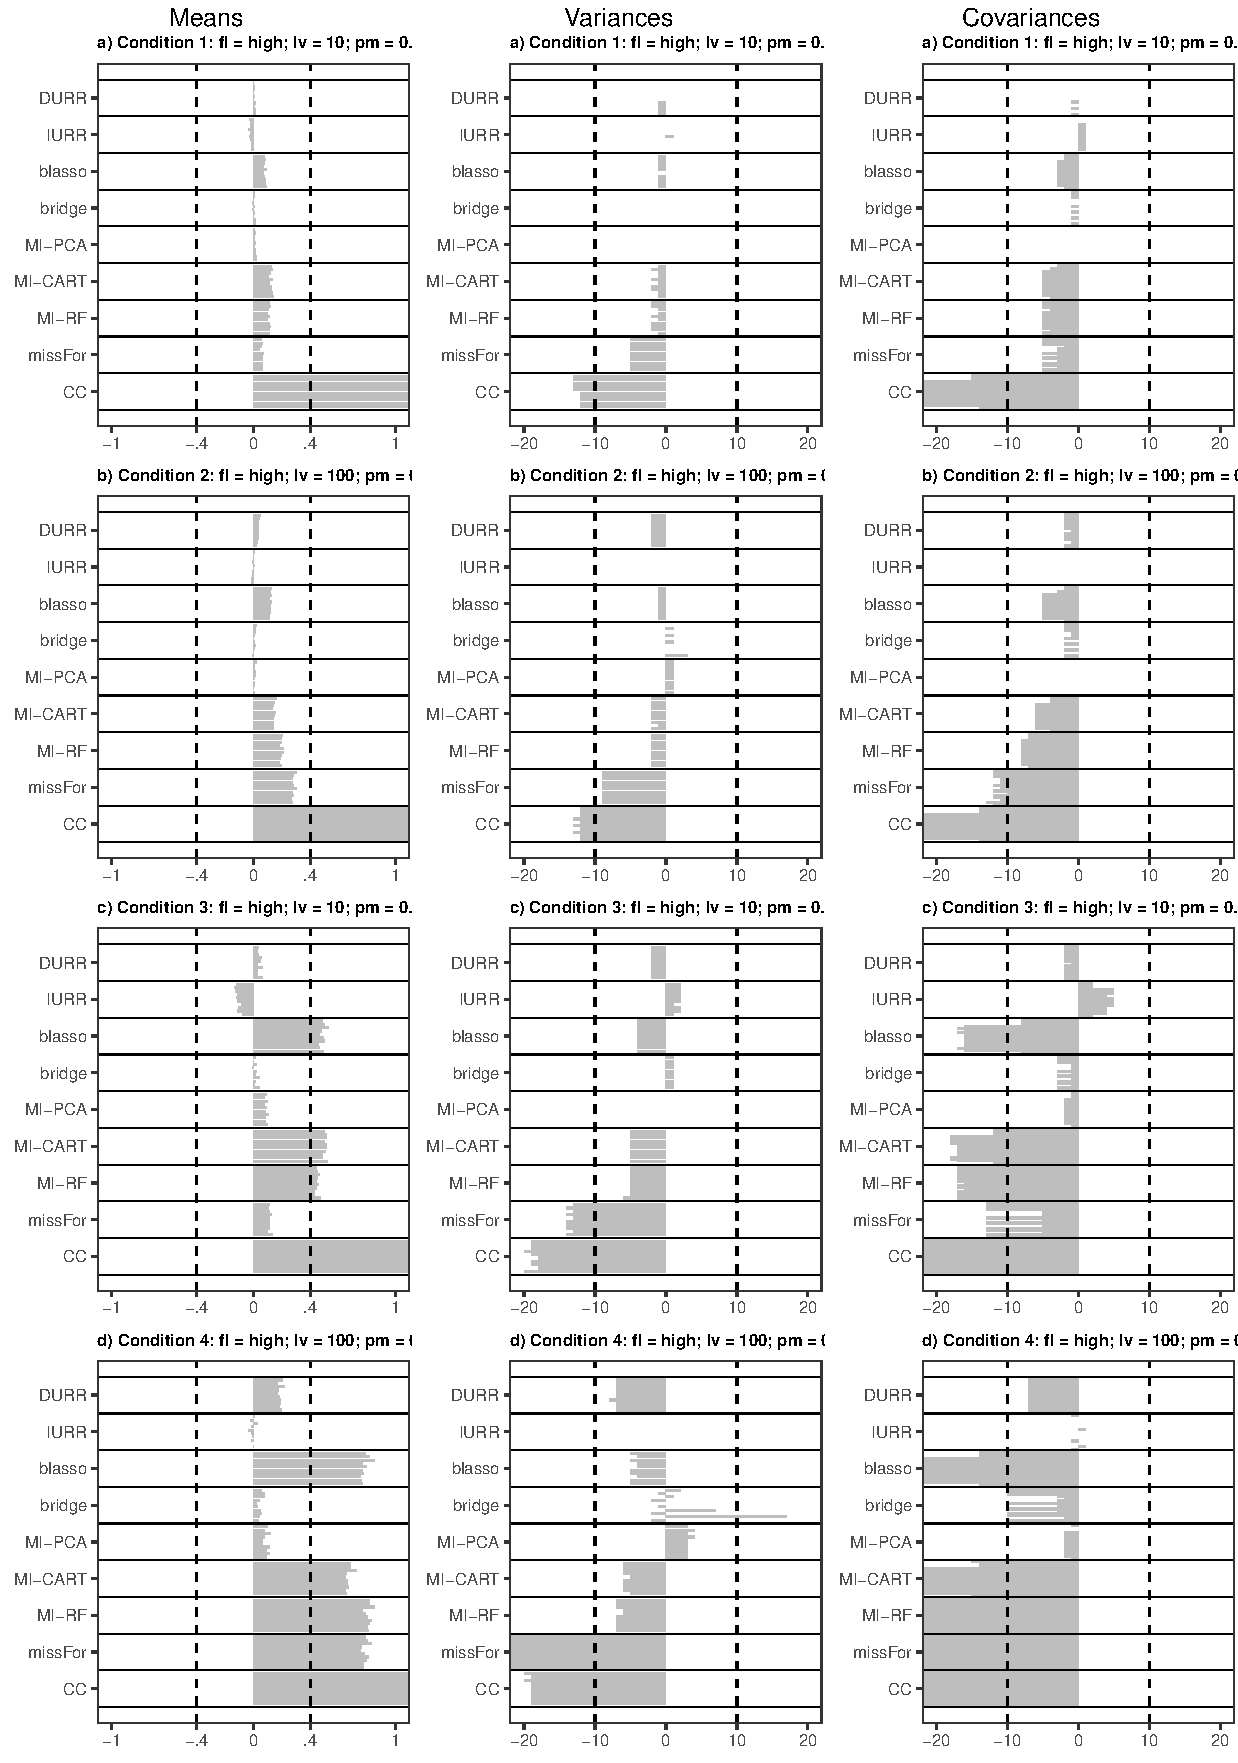
\includegraphics{\pathFIG/exp2_semR_bias_14.pdf}
\caption{PRBs for the means, variances and covariances (PRB) for condition 1 to 4.
	For every method, single horizontal lines, representing the PRB of a parameter estimate on 
	a single variable (or pair of variables), combine to form larger horizontal bars giving an 
	aggregate account of how each method performed across multiple variables with missing values.
}
\label{fig:exp2bias14}
\end{figure}

\begin{figure}
	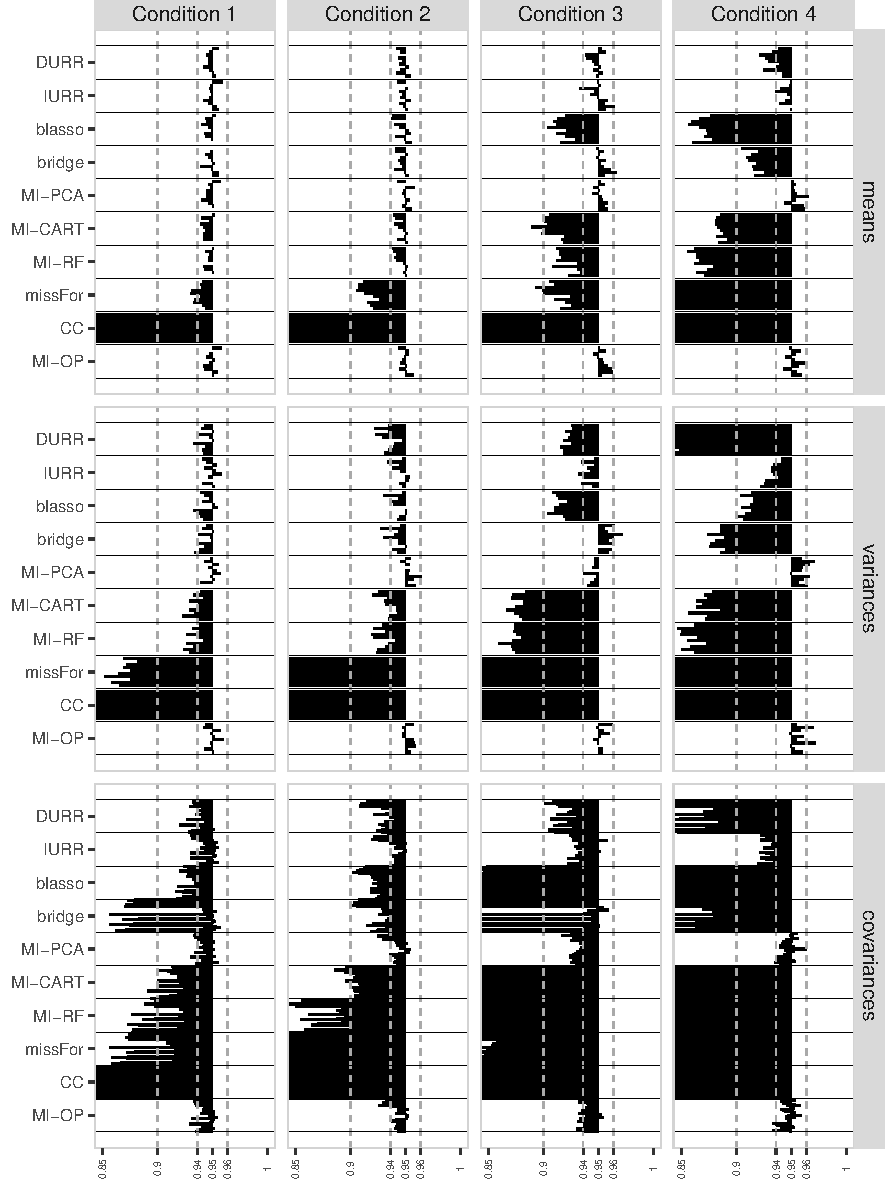
\includegraphics{\pathFIG/exp2_semR_ci_14.pdf}
\caption{CIC for the means, variances, and covariances for condition 1 to 4.
	For every method, single horizontal lines, representing the CIC of a parameter estimate on 
	a single variable (or pair of variables), combine to form larger horizontal bars giving an 
	aggregate account of how each method performed across multiple variables with missing values.
}
\label{fig:exp2cir14}
\end{figure}


\begin{figure}
	\centering
	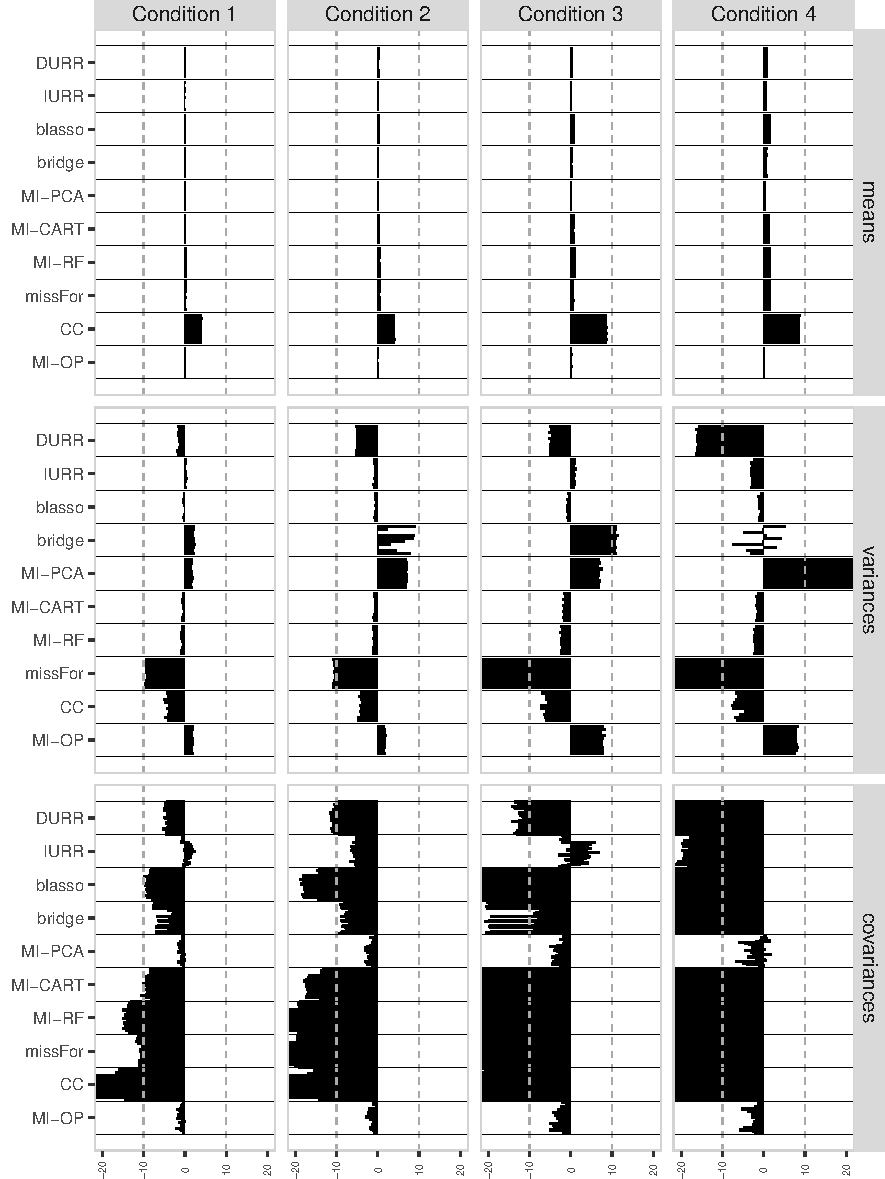
\includegraphics{\pathFIG/exp2_semR_bias_58.pdf}
	\caption{Bias estimation for the means (SB), variances and covariances (PRB) for condition 5 
			to 8.}
	\label{fig:exp2bias58}
\end{figure}

\begin{figure}
	\centering
	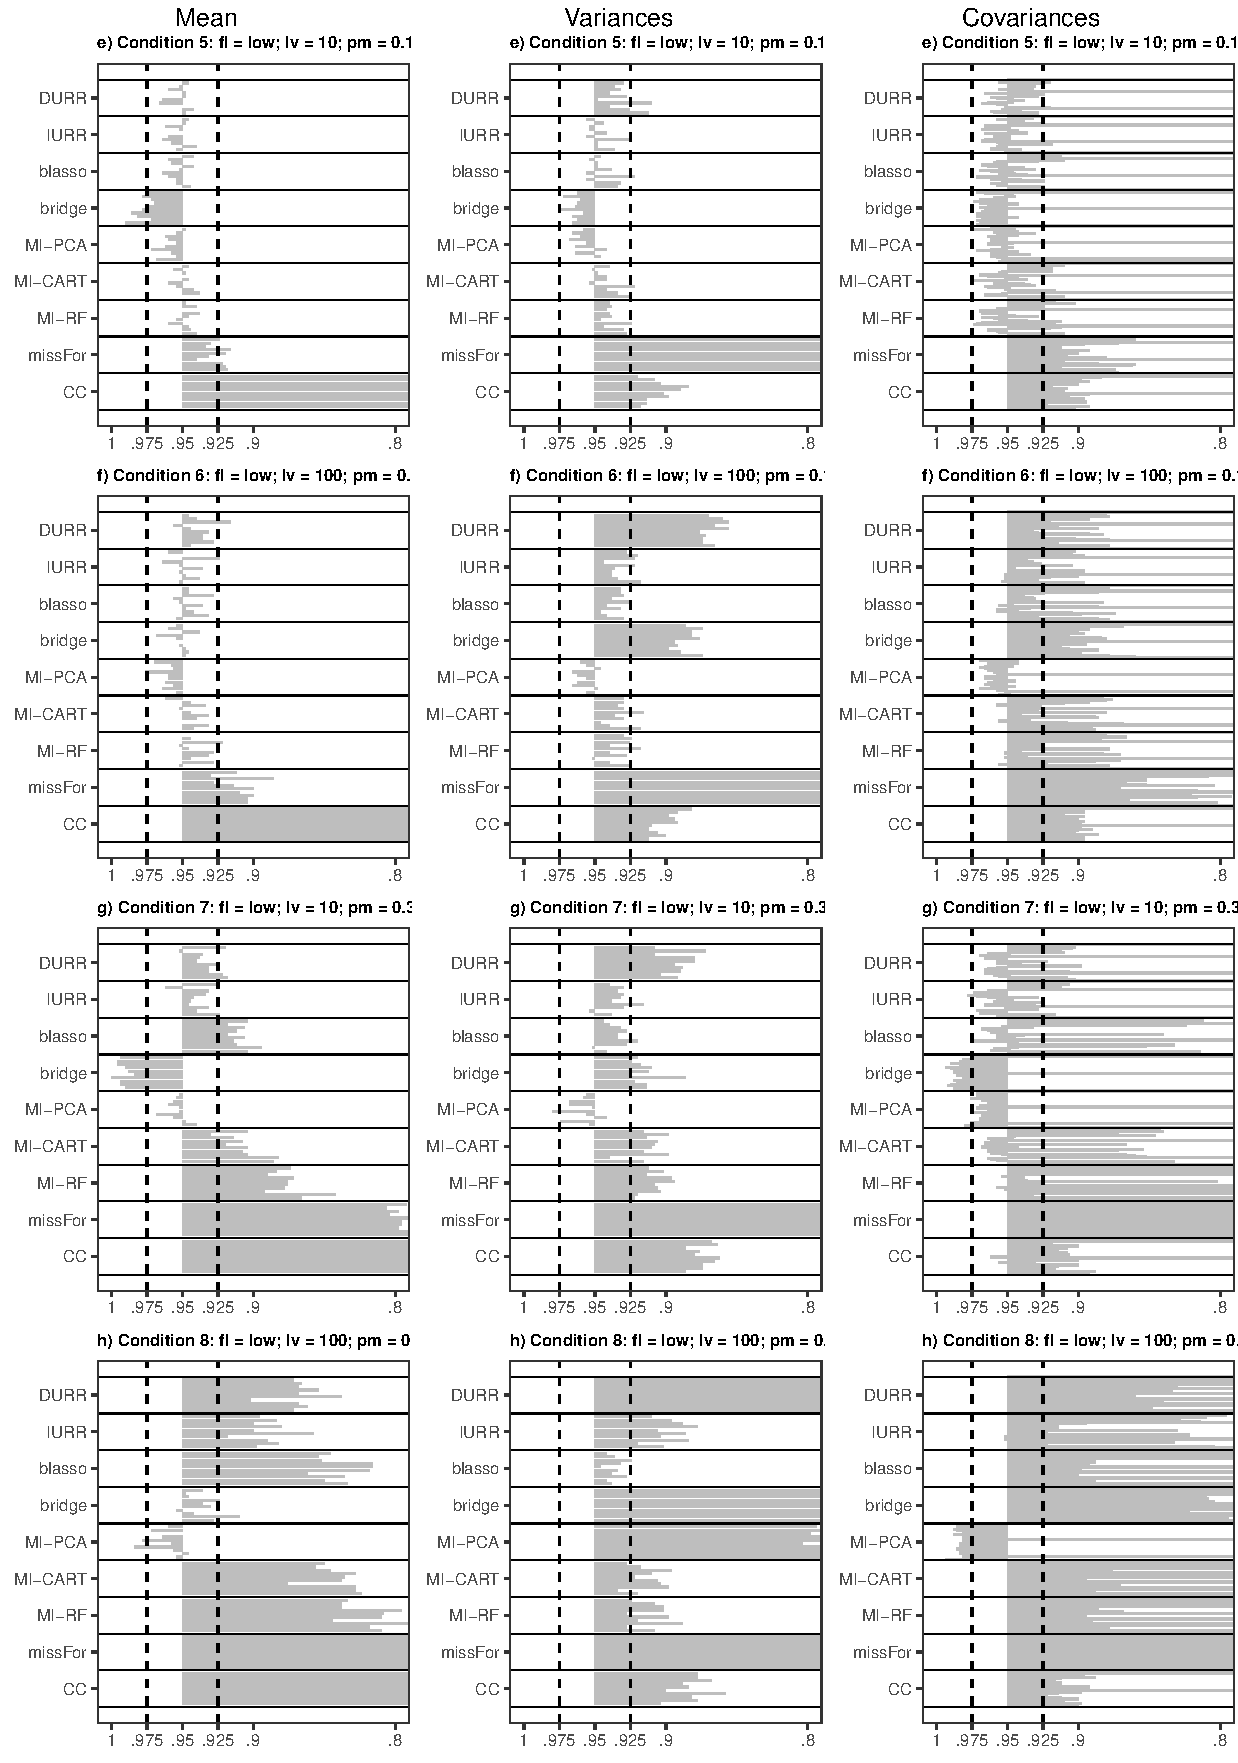
\includegraphics{\pathFIG/exp2_semR_ci_58.pdf}
	\caption{Confidence Interval Coverage (CIC) for the means, variances, and covariances 
			for condition 5 to 8.}
	\label{fig:exp2cir58}
\end{figure}

\begin{figure}
	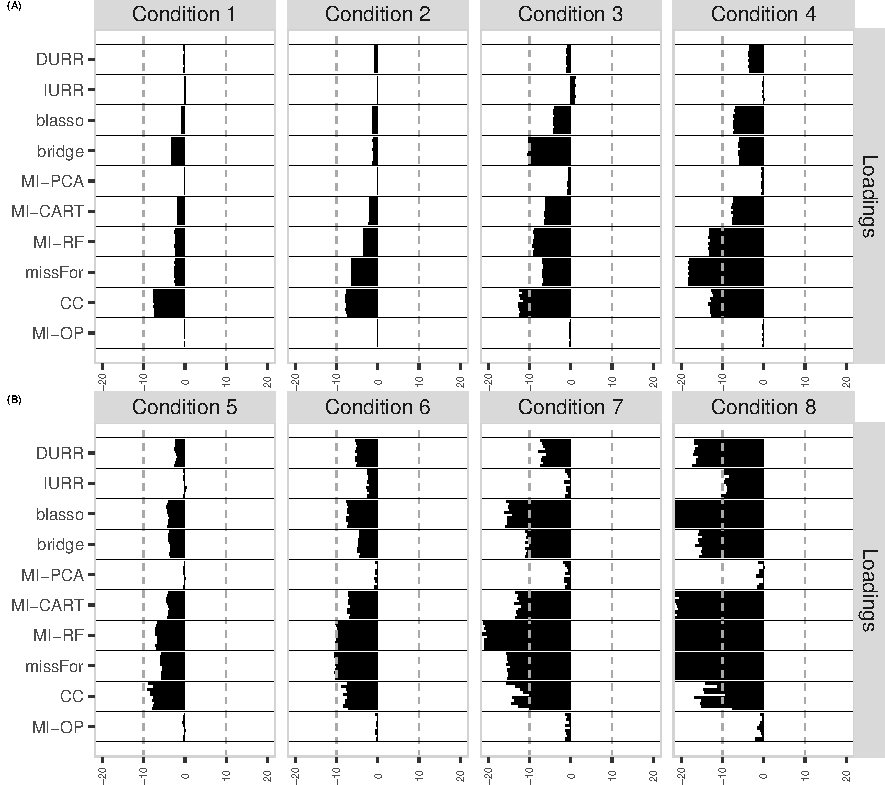
\includegraphics{\pathFIG/exp2_CFA_lambda_BPR.pdf}
	\caption{
		Percent Relative Bias (PRB) for the factor loadings in conditions 1 to 4 (panel A) 
		and conditions 5 to 8 (panel B).
		Within each panel, for every method, single horizontal lines report the PRB of the 
		factor loading estimation for each item with missing values.
		}
\label{fig:exp2flAll}
\end{figure}

\FloatBarrier

\subsection{Experiment 3: Resampling Study}

Supplements to resampling study

	Figure \ref{fig:exp4bias_m1} reports the absolute values of the PRBs for the intercept and all the partial 
	regression coefficients in Model 1, under the different imputation methods, for both the low- and high-dimensional
	conditions.
	Figure \ref{fig:exp4cir_m1} reports CIC results in the same way.

\begin{figure}
	\centering
	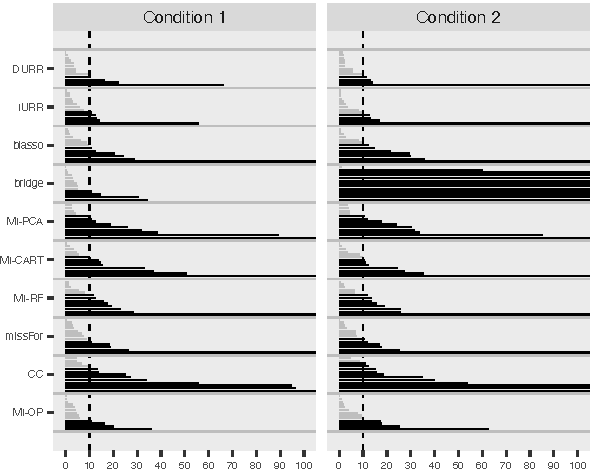
\includegraphics{\pathFIG/exp4_imp_bias_allParms_m1.pdf}
	\caption{PRBs for all the model parameters in model 1. 
		The order of the bars is based on the absolute value of the PRBs.
		The values for the intercept, the focal regression coefficient, and the regression coefficient with which most 
		methods struggle (Largest Bias) are highlighted}
	\label{fig:exp4bias_m1}
\end{figure}

\begin{figure}
	\centering
	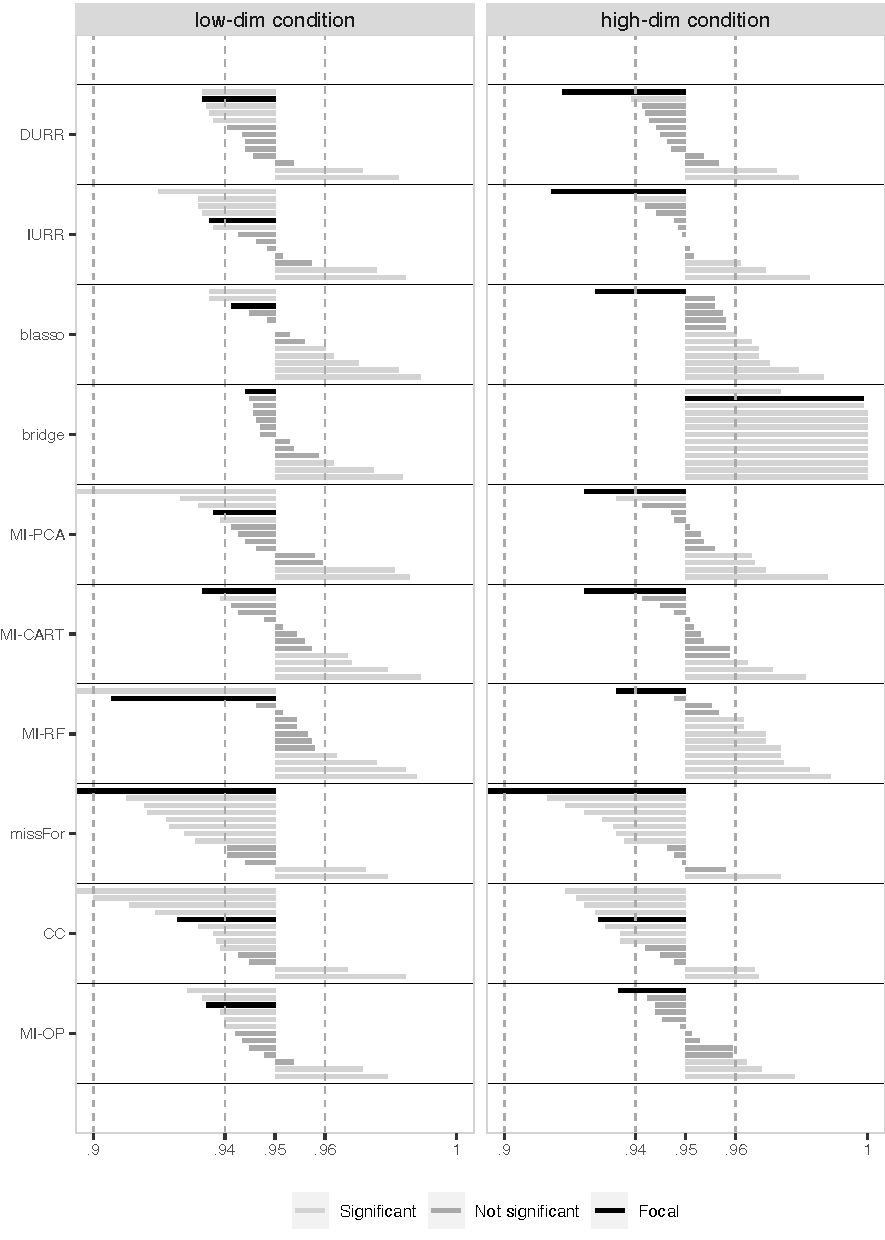
\includegraphics{\pathFIG/exp4_imp_ci_allParms_m1.pdf}
	\caption{CIC for all model parameter in model 1.
		Bars are sorted in by ascending value.
		The values for the intercept, the focal regression coefficient, and the regression coefficient with which most 
		methods struggle (Largest Bias) are highlighted}
	\label{fig:exp4cir_m1}
\end{figure}

\FloatBarrier

% Bibliography
\bibliographystyle{apacite} 

\bibliography{
	\pathBIB/missingData/bibtex/papers,
	\pathBIB/missingData/bibtex/books,
	\pathBIB/missingData/bibtex/software,
	\pathBIB/bayesStats/bibtex/papers,
	\pathBIB/programming/bibtex/papers,
	\pathBIB/survey/bibtex/data,
	\pathBIB/survey/bibtex/studies,
	\pathBIB/statsLearn/bibtex/books,	
	\pathBIB/statsLearn/bibtex/papers,
	\pathBIB/statsLearn/bibtex/software
	}

\end{document}
